\documentclass{article}
\renewcommand{\thesection}{\roman{section}} 
\usepackage{graphicx}
\usepackage[nottoc,numbib]{tocbibind}
\usepackage[a4paper, total={6in, 8.75in}]{geometry}
\usepackage{listings}
\usepackage{subcaption}
\usepackage{titling}
\usepackage{pgffor}
\newcommand{\subtitle}[1]{%
  \posttitle{%
    \par\end{center}
    \begin{center}\large#1\end{center}
    \vskip0.5em}%
}
\newcommand{\myparagraph}[1]{\paragraph{#1}\mbox{}\\}

\title{Topics in Privacy \& Security}
\subtitle{Trust-Enhanced Reputation Metrics}
\author{Y1481702}
\date{\today}
\setlength\parindent{0pt}
 
\begin{document}
\begin{titlepage}
\maketitle
\tableofcontents
\end{titlepage}

\lstset{
    tabsize=3,
    numbers=left,
    morekeywords={continue}
}

%Your report should not exceed four A4 pages (minimum font size 11pt), not counting the screenshots and plots from parts (ii) and (iii) of the question, and not counting the references.
%APPROX 1 page per 10 marks!

\section{Description} %5 Marks
%Describe how the tool works
%By means of pseudocode accompanied by a suitable description, explaining how your design takes into account scalability issues (so the tool can handle large input files)
In my implementation of the tool, a number of steps have been taken to help the tool scale.
The tool utilises relational databases to quickly access product rating data. \texttt{CUSTOMERS} and \texttt{PRODUCTS} as mentioned in the pseudocode are tables in the database. This means that the tool does not need to store all data in memory which is usually the most limited resource.
\\\\
As is visible from the pseudocode of the tool, I have also attempted to cut down on superfluous computation wherever possible.
\begin{lstlisting}
MAX_RATE, ALPHA, FILE = take input from user
CUSTOMERS, PRODUCTS = initialise empty array: []

for each RATING of PRODUCT_J by CUSTOMER_I in FILE:
	if RATING made by a new customer:
		CUSTOMERS.append(New CUSTOMER_I with Default Trust Level of 0.5)

	if RATING made of a new PRODUCT:
		PRODUCTS.append(New PRODUCT_J with RATING)
		continue to next RATING
	else:
		Update the Product Rating for PRODUCT_J

	for each CUSTOMER of PRODUCT_J in CUSTOMERS:
		Update the Trust Level of CUSTOMER

	for each PRODUCT bought by CUSTOMERS of PRODUCT_J:
		Update the Product Rating of PRODUCT

\end{lstlisting}

%FIND REFERENCES FOR significant scalability issues of Trust-Based Reputation Systems?
On Line 6 of the above pseudocode, Equation 3 (from the brief) always returns 0.5 when run with an empty set of products. There is no need to run this calculation equation each time, and not doing so will save us a small amount of compute time. On Line 10, in the case that this rating is for a new product, the algorithm skips the updating of related customers and products as this will have little effect. This is because, if a product only has one customer, its overall rating is the same as that customer's rating.
\\\\
The loops to update customer trust levels and product ratings on Lines 14 and 17 respectively, are kept to a minimum by filtering down to only updating trust levels of customers that bought the newly rated product. For efficiency, the final implementation need to take care to ensure that each of customer and product is updated only once. If required, further steps to reduce runtime that have not been taken in my implementation, could include only updating Product Ratings (Line 18) if the customer trust levels have changed significantly and running trust level (Line 15) and product rating (Line 18) updates in different, parallel threads.
\\\\
As systems scale, they are more likely to become the target of a form of cyber attack. Prepared statements have been used to sanitise inputs whenever input data from outside the program's control is entered into the database in order to protect against SQL injection attacks.

\section{Analysis} %15 Marks
%Use the tool with MAX_RATINGS=5 to analyse the effect of using \alpha=1, \alpha=1.5, \alpha=2 and \alpha=5 on the overall product ratings from the input file Q2Ratings.txt.

%Include screenshots of the tool output;
\ref{fig:tool_output}

%and plots of the overall ratings of the products with IDs 4, 7 and 29 for these \alpha values.


%Discuss the differences between the results obtained for different \alpha values, and between these results and the results obtained for the arithmetic mean.

\section{Simulated Attacks} %10 Marks
%Simulate a self-promoting attack to improve the rating of the product with ID 4 by adding n fake top ratings for this product at the end of Q2Ratings.txt from part (ii) of the question. Each such rating should have a new customer ID, corresponding to a new customer account created by the attacker(s).
Self-promoting attacks of varying sizes have been simulated on product \#4, this is shown by Fig. \ref{fig:graph_promote}.
%Plot the increase in the overall rating achieved by attacks of size n=5, n=10, n=15, n=20 and n=25 for the four \alpha values from part (ii) of the question and for an overall rating based on the arithmetic mean.
%Repeat the experiments for slandering attacks on product with ID 29, plotting the decrease in the overall rating achieved by slandering attacks of size n=5, n=10, n=15, n=20 and n=25 for the four \alpha values from part (ii) of the question and for an overall rating based on the arithmetic mean.
Slander attacks of varying sizes have been simulated on product \#29, this is shown by Fig. \ref{fig:graph_slander}.

\section{Results}
%Discuss the results from part (iii) of the question. Explain what value of the parameter \alpha offers the best protection against the attacks you experimented with, and assess the advantages and disadvantages	of different values for \alpha.
The results show that the system is least susceptible to attack when an $\alpha$ value of 2 is used.
Using values of alpha that ignore new reviews may prevent genuine customer reviewers' opinions from being heard.

\newpage
\raggedright
\bibliography{Report}{}
\bibliographystyle{ieeetran}
\newpage
\section{Appendix}
%You must attach as an appendix to your single-file submission the source code for the tool. If needed, use a ZIP archive to submit all components of the assessment as a single file.
\begin{figure}[ht]
\centering
\begin{subfigure}{0.5\textwidth}
\centering
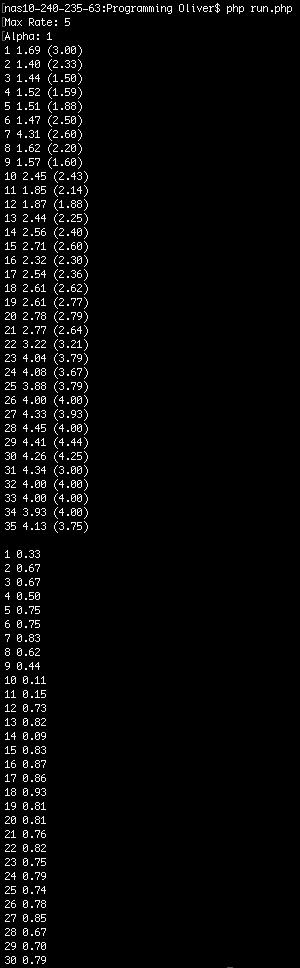
\includegraphics[width=0.675\textwidth]{Screenshots/Alpha1}
\caption{$\alpha = 1$}
\label{fig:screen_alpha1}
\end{subfigure}%
\begin{subfigure}{0.5\textwidth}
\centering
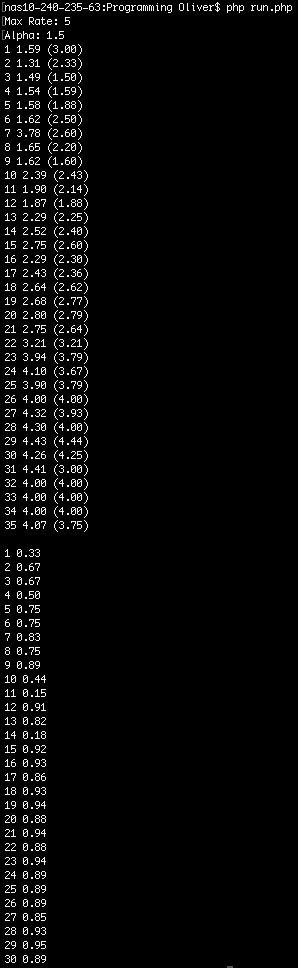
\includegraphics[width=0.675\textwidth]{Screenshots/Alpha1_5}
\caption{$\alpha = 1.5$}
\label{fig:screen_alpha1.5}
\end{subfigure}
\end{figure}

\begin{figure}\ContinuedFloat
\begin{subfigure}{0.5\textwidth}
\centering
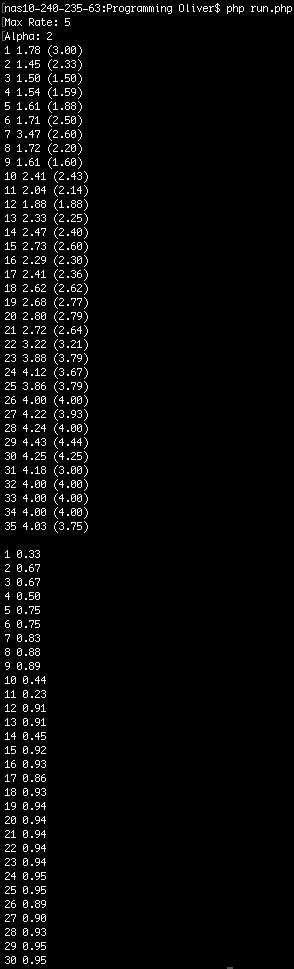
\includegraphics[width=0.70\textwidth]{Screenshots/Alpha2}
\caption{$\alpha = 2$}
\label{fig:screen_alpha2}
\end{subfigure}%
\begin{subfigure}{0.5\textwidth}
\centering
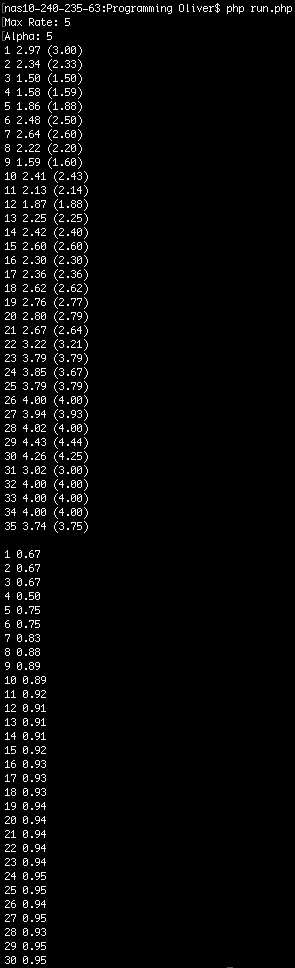
\includegraphics[width=0.70\textwidth]{Screenshots/Alpha5}
\caption{$\alpha = 5$}
\label{fig:screen_alpha5}
\end{subfigure}
\caption{Tool Output for Varying Alpha}
\label{fig:tool_output}
\end{figure}

\begin{figure}[ht]
\centering
\begin{subfigure}{0.85\textwidth}
\centering
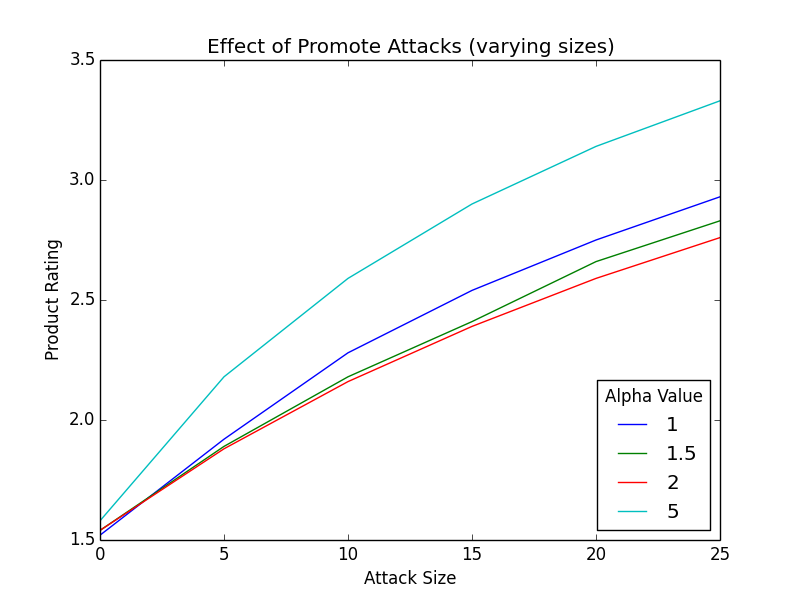
\includegraphics[width=1\textwidth]{Graphs/Promote}
\caption{Effect of Self-Promotion Attacks of Varying Sizes on Product 4}
\label{fig:graph_promote}
\end{subfigure}
\begin{subfigure}{0.85\textwidth}
\centering
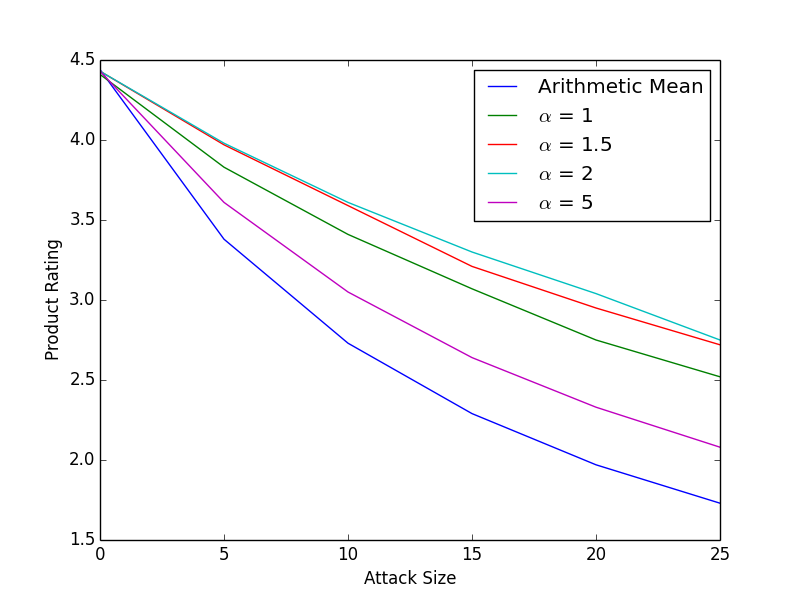
\includegraphics[width=1\textwidth]{Graphs/Slander}
\caption{Effect of Slander Attacks of Varying Sizes on Product 29}
\label{fig:graph_slander}
\end{subfigure}
\caption{Attacks on the Online Store Rating System}
\end{figure}

\foreach \x in {run, attack, setup, process, output}
{
	\subsection{\x.php}
	\lstinputlisting[language=PHP]{Programming/\x.php}
}

\end{document}